\documentclass{idrisMemo}

\memoto{Idris}
\memosubject{Book of Proof}
\memodate{2024.03.10}
\status{\S 3.5 Counting Subsets}

\begin{document}
\toc

\begin{prooflist}{1. What is the smallest n for which n! has more than 10 digits?}
    \item If a number is 10 digits, then it must be more than $10^{9}$.
    \item 13
\end{prooflist}

\begin{prooflist}{1. Suppose a set A has 37 elements}
\item How many subsets of A have 10 elements?
\item $\dbinom{37}{10} = \dfrac{37!}{27! \cdot10!}$
\item How many subsets have 30 elements?
\item $\dbinom{37}{30} = \dfrac{37!}{30! \cdot7!}$
\item How many have 0 elements?
\item $\dbinom{37}{0} = \dfrac{37!}{0! \cdot37!}=1$
\end{prooflist}

\begin{prooflist} {2. Suppose A is a set for which $|A| = 100$.}
\item How many subsets of A have 5 elements?
\item $\dbinom{100}{5} = \dfrac{100!}{5! \cdot95!}$
\item How many subsets have 10 elements?
\item $\dbinom{100}{10} = \dfrac{100!}{10! \cdot90!}$
\item How many have 99 elements?
\item $\dbinom{100}{99} = \dfrac{100!}{99! \cdot1!}= 100$
\end{prooflist}

\begin{prooflist}{3. A set X has exactly 56 subsets with 3 elements. What is the cardinality of X?}
\item $\dbinom{a}{3} = \dfrac{a!}{3! \cdot(a-3)!}=56$, for some $a \in \mathbb{N}$.
\item $\dfrac{(a)(a-1)(a-2)}{6}=56$
\item $(a)(a-1)(a-2)=336$
\item $a(a^2-3a+2)=336$
\item $a^3-3a^2+2a=336$
\item $a^3-3a^2+2a-336=0$
\item via the rational root theorem, $a=8$.
\end{prooflist}

\begin{prooflist}{4. Suppose a set B has the property that}
    \item $$|\{X: X \in \mathcal{P}(B),\quad|X|=6\}|=28$$
    \item Find $|B|$.
    \item B is set such that there 28 subset elements of its powerset that have
        6 elements.
    \item $\dbinom{a}{6}=28 = \dfrac{a!}{6!\cdot(a-6)!}$
    \item $\dfrac{a(a-1)(a-2)(a-3)(a-4)(a-5)}{6!}=28$
    \item $a(a-1)(a-2)(a-3)(a-4)(a-5)=28\cdot6!$
    \item through trial and error, $a=8$.
\end{prooflist}

\begin{prooflist}{5. How many 16-digit binary strings contain exactly seven
    1’s?}
\item Examples
\item 0111000011110000
\item 0011001100110010
\item $\dbinom{16}{7}= \dfrac{16!}{7!\cdot9!}$
\end{prooflist}

\begin{prooflist} { 6. $|\{X \in \mathcal{P}(\{0,1,2,3,4,5,6,7,8,9\}):|X|=4\}|=?$}
\item $X$ is a set-element of the powerset of the set comprising the digits
    0..9.
\item $\dbinom{10}{4}= \dfrac{10!}{6!\cdot4!}=210$
\end{prooflist}

\begin{prooflist} { 7. $|\{X \in \mathcal{P}(\{0,1,2,3,4,5,6,7,8,9\}):|X|<4\}|=?$}
\item $X$ is a set-element of the powerset of the set comprising the digits
    0..9.
\item $\dbinom{10}{3} + \dbinom{10}{2} + \dbinom{10}{1} + \dbinom{10}{0}$
\end{prooflist}

\begin{prooflist}{8. This problem concerns lists made from the symbols A, B, C, D, E, F, G, H, I.}
\item (a) How many length-5 lists can be made if there is no repetition and the
    list is in alphabetical order? (Example: BDEFI or ABCGH, but not BACGH.)
\item There is an equivalent problem where we choose 5 letters without
    replacement. Each such list has a distinct ordering, which is equivalent to
    a sorted list without replacement.
\item Therefore the answer is $\binom{8}{5}=56.$
\item (b) How many length-5 lists can be made if repetition is not allowed and
    the list is not in alphabetical order?
\item Here we do not consider each set of the same letters as unique, so we can
    just the multiplication principle and the answer is $\dfrac{8!}{3!}$.
\end{prooflist}

\begin{prooflist}{9. This problem concerns lists of length 6 made from the
    letters A,B,C,D,E,F, without repetition. How many such lists have the
    property that the D occurs before the A?}
\item It is equally likely that D appears before the A as it is the D appears
    after the A.
\item The number of possible lists is $6!$, and the number of possible list
    where the D appears before the A is $\dfrac{6!}{2}$.
\end{prooflist}

\begin{prooflist}{10. A department consists of 5 men and 7 women. From this
    department you select a committee with 3 men and 2 women. In how many ways
    can you do this?}
\item There $\dbinom{5}{3}$ to choose the men, and $\dbinom{7}{2}$ to choose the
    women.
\item Therefore there are $\dbinom{5}{3}\cdot \dbinom{7}{2}$ ways to create the
    committee.
\end{prooflist}

\begin{prooflist}{11. How many positive 10-digit integers contain no 0’s and exactly three 6’s?}
\item First let us determine the slots where the 6s can go. There are 10 slots,
    thus the 6s can go in $\binom{10}{3}$ spots.
\item Next let us determine the number of digits comprised of 1..5,7..9 that
    are length-7. Since the set has 8 digits, the answer is $8^7$.
\item Thus by the multiplication principle, where there $8^{7}\cdot\binom{10}{3}$ possibilities.
\end{prooflist}

\begin{prooflist}{12. Twenty-one people are to be divided into two teams, the
    Red Team and the Blue Team. There will be 10 people on Red Team and 11
    people on Blue Team. In how many ways can this be done?}
\item Determining one team fully determines the other team. We can use this idea
    to see if we get the same answer, depending on which team is formed first.
\item To form the blue team, there are $\dbinom{21}{11}$ possibilities.
\item To form the red team, there are $\dbinom{21}{10}$ possibilities.
\item $\dbinom{21}{10} = \dfrac{21!}{10!\cdot11!} = \dbinom{21}{11}$, thus we
    can see that forming either team first results in the same answer.
\end{prooflist}

\begin{prooflist}{13. Suppose $n, k \in \mathbb{Z}$, and $0 \leq k \leq n$. Use
    Fact 3.5, the formula $\left(\begin{array}{c}n \\
    k\end{array}\right)=\dfrac{n !}{k !(n-k) !}$, to show that
$\left(\begin{array}{l}n \\ k\end{array}\right)=\left(\begin{array}{c}n \\
n-k\end{array}\right)$.}
\item $\dbinom{n}{k}=\dfrac{n!}{k!(n-k)!}$
\item
    $\dbinom{n}{n-k}=\dfrac{n!}{(n-k)(n-(n-k))!}=\dfrac{n!}{(n-k)!(n-n+k)!}=\dfrac{n!}{(n-k)!k!}$
\end{prooflist}

\begin{prooflist}{14. Suppose $n, k \in \mathbb{Z}$, and $0 \leq k \leq n$. Use Definition 3.2 alone (without using Fact 3.5) to show that $\left(\begin{array}{l}n \\ k\end{array}\right)=\left(\begin{array}{c}n \\ n-k\end{array}\right)$.}
\item Suppose some set of cardinality $n$.  Suppose any $k$ such that $0 \leq k \leq n$.
\item Now we partition $n$ into $k$ and $n-k$ elements. There are two
    equivalent ways of creating this partition, either by selecting $k$ or
    selecting $n-k$ elements.
\item Therefore $\dbinom{n}{k}$ is equivalent to $\dbinom{n}{n-k}$.
\end{prooflist}

\begin{figure}
   \centering
   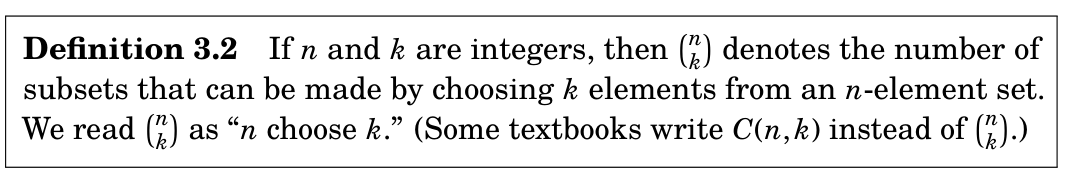
\includegraphics[width=0.9\textwidth]{images/definition03_02.png}
   \label{fig:mypicture}
\end{figure}

\begin{prooflist}{15. How many 10-digit binary strings are there that do not have exactly four 1’s?}
    \item Let $A=$ set of all 10-digit binary strings.
    \item Let $B=$ set of all 10-digit binary strings with exactly four 1's.
    \item Let $C=$ set of all 10-digit binary strings that do not have exactly
        four 1's.
    \item Because B and C are complements and A is the universe of all 10-digit
        binary strings, then $B \cup C = A$ and $|A|-|B| = |C|$.
    \item Using the multiplication principle, we determine $|A|$ is $2^{10}$.
    \item For $B$, there are 4 spots out of 10 where we can place 1s. Therefore
        \mbox{$|B|=\binom{10}{4}$}.
    \item Therefore $|C|=2^{10} - \binom{10}{4}$.
\end{prooflist}

\begin{prooflist}{16. A = $\{ 0,1,2,3,4,5,6,7,8,9\}$}
    \item Let $B=$ Even elements of A.
    \item Let $C=$ Odd elemements of A.
    \item Let $D=$ 6-elements subsets of A that have exactly 3 even elements.
    \item Let $E=$ 6-elements subsets of A that do not have exactly 3 even elements.
\item How many 6-element subsets of A have exactly three even elements?
    \item We can first choose 3 elements from B, and then choose 3 elements of
        C, and combine them together with the multiplication principle.
    \item $|B| = |C| = \dbinom{5}{3}$, and therefore $|D| = {\dbinom{5}{3}}^2$.
\item How many do not have exactly three even elements?
\item E is the complement of D, therefore $|E| = \dbinom{10}{6} -
    {\dbinom{5}{3}}^2$.
\end{prooflist}

\begin{prooflist}{ Let $A$ be the set of 10-digit binary strings. }
    \item Let $B=$ subset of A with exactly four 1's
    \item Let $C=$ subset of A with exactly five 1's
    \item Let $D=$ subset of A whose elements have exactly four 1’s or exactly five 1’s
    \item Let $E=$ subset of A whose elements do not have exactly four 1’s or exactly five 1’s
    \item How many elements of A are there that have exactly four 1’s or exactly five 1’s?
    \item Because $B \cap C=\emptyset$, B and C partition D. Therefore, we can
        calculate the cardinalities separately and then add them.
    \item $|B|=\binom{10}{4}$ and $|C|=\binom{10}{5}$, $|D|= \binom{10}{4}+\binom{10}{5}$.
    \item How many do not have exactly four 1’s or exactly five 1’s?
    \item $E$ is the complemenet of D, therefore $|E| = |A| - |D| = 2^{10} -
        \binom{10}{4}-\binom{10}{5}$.
\end{prooflist}

\begin{prooflist}{18. How many 10-digit binary strings have an even number of 1’s?}
    \item Let $A$ be the set of 10-digit binary strings.
    \item Let $B=$ subset of A with exactly 0 1's
    \item Let $C=$ subset of A with exactly 2 1's
    \item Let $D=$ subset of A with exactly 4 1's
    \item Let $E=$ subset of A with exactly 6 1's
    \item Let $F=$ subset of A with exactly 8 1's
    \item Let $G=$ subset of A with exactly 10 1's
    \item Let $H=$ subset of A with an even number of 1's
    \item Because B, C, D, E, F, and G partition H, $H=B\cup C\cup D\cup E \cup
        F \cup G$, and therefore $|H|=|B| + |C| + |D| + |E| + |F| + |G|$.
    \item Because of the equivalance of $\binom{n}{k}$ and $\binom{n}{n-k}$,
        $|B|=|G|, |C|=|F|, |D|=|E|$.
    \item Therefore $|H| =
        2\cdot \binom{10}{0} +
        2\cdot \binom{8}{2} +
        2\cdot \binom{6}{4}$.
\end{prooflist}

\begin{prooflist}{19. A 5-card poker hand is called a flush if all cards are the same suit. How many different flushes are there?}
\item To get a flush of one particular suit, we choose 5 cards from a set of 13,
    which equals $\dbinom{13}{8}$.
\item Because there are 4 different suits in the deck of card, we have 4 ways of
    getting the flush and the total number of flush possibilities is $4 \cdot
    \dbinom{13}{8}$.
\end{prooflist}

\end{document}
